\section{Testing}

Every embedded system needs to be tested. Generally, it is also valuable or mandatory that testing be performed at several levels. The most common levels of testing are:

\begin{itemize}
    \item System tests verify that the product as a whole meets or exceeds the stated requirements. System tests are generally best developed outside of the engineering department, though they may fit into a test harness developed by engineers. \textbf{The system tests should treat the firmware as a black box.}
    
    \item Integration tests verify that a subset of the subsystems identified in the architecture diagrams interact as expected and produce reasonable outcomes. Integration tests are generally best developed by a testing group or person within software engineering.
    
    \item Unit tests verify that individual software components identified at the intermediate design level perform as their implementers expect. That is, they test at the level of the public API the component presents to other components. Unit tests are generally best developed by the same people that write the code under test. \textbf{Proponents of test-driven development advocate that tests at this level be written in advance of the functions or classes that they are intended to verify.}
\end{itemize}

Of the three, system tests are most easily developed, as those test the product at its exposed hardware interfaces to the world (e.g., does the dialysis machine perform as required). Of course, a test harness may need to be developed for engineering and/or factory acceptance tests. But this is generally still easier than integration and unit tests, which demand additional visibility inside the device as it operates.

To make the development, use, and maintenance of integration and unit tests easy, it is valuable to architect the firmware in a manner compatible with a software test framework. The single best way to do this is to architect the interactions between all software components at the levels you want to test so they are based on publish-subscribe event passing (a.k.a., message passing).

Interaction based on a publish-subscribe model allows a lightweight test framework like the one shown in Figure 2 to be inserted alongside the software component(s) under test. Any interface beween the test framework and the outside world, such as a serial port, provides an easy way to inject or log events. A test engine on the other side of that communications interface can then be designed to accept test “scripts” as input, log subscribed event occurrences, and off-line check logged events against valid result sequences. Adding timestamps to the event logger and scripting language features like delay(time) and waitfor(event) significantly increases testing capability.

\begin{figure}[h!]
\centering
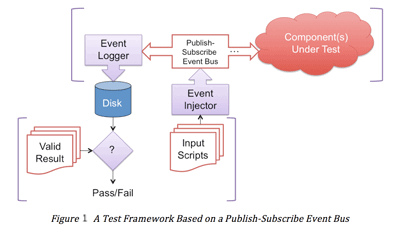
\includegraphics[scale=0.8]{./images/testing_procedure}
\end{figure}

It is unfortunate that the publish-subscribe component interaction model is at odds with proven methods of analyzing software schedulability (e.g., RMA). The sheer number of possible message arrival orders, queue depths, and other details make the analysis portion of guaranteeing timeliness difficult and fragile against minor implementation changes. This is, in fact, why it is important to separate the code that must meet deadlines from the rest of the software. In this architecture, though, the real-time functionality remains difficult to test other than at the system level.